\documentclass[a4paper,10.5pt]{ltjsarticle}
\usepackage{graphicx}
\usepackage{luatexja-fontspec}
\usepackage{caption}
\usepackage{amsmath,amssymb,bm,braket}
\usepackage{gnuplot-lua-tikz}
\usepackage[top=10truemm,bottom=15truemm,left=10truemm,right=10truemm]{geometry}
\usepackage{array}
\usepackage{upgreek}
\usepackage{fancybox}
\usepackage{fancyhdr}
\renewcommand{\refname}{}
\usepackage{listings,jvlisting}
\usepackage{tikz}
\usetikzlibrary{external}
\tikzexternalize
\lstset{
  basicstyle={\ttfamily},
  identifierstyle={\small},
  commentstyle={\smallitshape},
  keywordstyle={\small\bfseries},
  ndkeywordstyle={\small},
  stringstyle={\small\ttfamily},
  frame={tb},
  breaklines=true,
  columns=[l]{fullflexible},
  numbers=left,
  xrightmargin=0pt,
  xleftmargin=3pt,
  numberstyle={\scriptsize},
  stepnumber=1,
  numbersep=1pt,
  lineskip=-0.5ex
}
\captionsetup[figure]{format=plain, labelformat=simple, labelsep=quad,labelfont=bf}
\captionsetup[table]{format=plain, labelformat=simple, labelsep=quad,labelfont=bf}
\parindent = 0pt
\setmainjfont[BoldFont=HiraMinProN-W6]{HiraMinPro-W3}
%[BoldFont=HGSMinchoE]{MSMincho}[BoldFont=HiraMinProN-W6]{HiraMinPro-W3}
\begin{document}
\centerline{\huge\bfseries アルゴリズムとデータ構造 理解度確認レポート(前半)}
\centerline{\ }
\rightline{\large 学籍番号:62115799}
\rightline{\large 氏名:平井優我}
{\large\bfseries [基礎問題01-01]}\\
 まず、$4x^2-9=0$の方程式の解は、
\begin{align}
  x=\pm\frac{3}{2}
\end{align}
となる。ニュートン法によってこの解のどちらかが得られることを示す。整数$n\geq 0$を用いて、$n$番目の$x$軸との切片を$x_n$とおく。このとき解析的に以下のような漸化式が求まる(ただし、初期値が$0$のときはニュートン法を用いても切片がもとまらないことは自明)。
\begin{align}
  x_{n+1}=\frac{1}{2}\left(x_n+\frac{9}{4}\frac{1}{x_n}\right)\ ,\ (x_n\neq 0)
\end{align}
今、$x_n>0$のとき$x_{n+1}>0$、$x_n<0$のとき$x_{n+1}<0$となる。また、$x_n>0$だとして(2)式の両辺に$-1$をかけると、その漸化式は$x_n<0$としたときと同じ式を表す。これより、$x_n>0$だとして得られた議論について、$x_n$の符号を逆にすれば$x_n<0$のときの議論が再現できることがわかる。よって、これ以降は$x_n>0$の範囲のみで議論する。\\
 まず、$x_n$と$x_{n+1}$の符号は一致することから、必ず$x_n\neq 0$である。(2)式の$x_n,x_{n+1}$をすべて$\alpha$に置き換えて$x$について解くと、
\begin{align}
  \alpha&=\frac{1}{2}\left(\alpha+\frac{9}{4}\frac{1}{\alpha}\right)\\
  \therefore\ \alpha&=\frac{3}{2}\ \ (x_n<0のときは負の解をとる。)
\end{align}
と求まる。(2)式から(3)式を引くと、
\begin{align}
  x_{n+1}-\alpha=\frac{1}{2}(x_n-\alpha)+\frac{9}{8}\left(\frac{1}{x_n}-\frac{1}{\alpha}\right)
\end{align}
となる。ここで、重要となるのは(5)式右辺の第2項の符号である。$x_{n+1}>0$、$x_n>0$であることから、(2)式について相加・相乗平均を用いると、
\begin{align}
   x_{n+1}&=\frac{1}{2}\left(x_n+\frac{9}{4}\frac{1}{x_n}\right)\nonumber\\[10pt]
  &\geq\sqrt{\frac{9}{4}}=\frac{3}{2}
\end{align}
となる。これは、どのような初期値を持ってきたとしても$x_1$以降は必ず3/2以上になることを表している。よって、$n\geq 1$について、(5)式右辺の第2項の符号は負となり、
\begin{align}
  |x_{n+1}-\alpha|\leq\frac{1}{2}|x_n-\alpha|
\end{align}
が成り立つ。(7)式を繰り返し用いることによって、
\begin{align}
  |x_n-\alpha|\leq\frac{1}{2^{n-1}}|x_1-\alpha|
\end{align}
となる。よって、$n\rightarrow\infty$としてはさみうちの原理から、
\begin{align}
  \lim_{n\rightarrow\infty}x_n=\alpha=\frac{3}{2}
\end{align} 
となる。これは、(1)で求めた正の解と一致する。\\
 以上をまとめると、
\clearpage
\begin{table}[h]
  \newcolumntype{I}{!{\vrule width 1.5pt}}
  \newcolumntype{i}{!{\vrule width 0.5pt}}
  \arrayrulewidth=0.8pt
  \renewcommand{\arraystretch}{1.5}
  \newcommand{\bhline}[1]{\noalign{\hrule height #1}}
  \centering
  \begin{tabular}{IcicI}
    \bhline{1.5pt}
    初期値&求まる解\\
    \bhline{1.0pt}
    正&$\frac{3}{2}$\\
    \hline
    負&$-\frac{3}{2}$\\
    \hline
    0&求まらない\\
    \bhline{1.5pt}
  \end{tabular}
\end{table} 
となる。\\
\\
{\large\bfseries [基礎問題02-01]}\\
 2進数表示したい10進数の数を$b$とすると、$b$を2で$n$回割ったときの商を$b_n$、余りを$d_n$とする。$b$を2進数表示するということは、
\begin{align}
  b=a_02^0+a_12^1+a_22^2+\cdots
\end{align}
というふうに表すことと同値である。$b,b_n$を2で割ったときの商と余りで表すと、
\begin{gather}
  b=2b_0+d_0\nonumber\\
  b_0=2b_1+d_1\nonumber\\
  b_1=2b_2+d_2\nonumber\\
  \vdots\nonumber\\
  b_{n-2}=2b_{n-1}+d_{n-1}\\
  b_{n-1}=2\cdot 0+d_{n}
\end{gather}
となる。ただし$b_{n}=0$となるまで繰り返す。(12)式を1つ前の(11)式へ代入し、得られた式を次々とその1つ前の式に代入していくと、
\begin{align}
  b=d_02^0+d_12^1+d_22^2+\cdots+d_n2^n
\end{align}
と表せることがわかる。よって、$a_i=d_i$とすることによって、bを2進数で表すことができる。\\
 次の表に20231201について、$d_i$を示す。
\begin{table}[h]
  \newcolumntype{I}{!{\vrule width 1.5pt}}
  \newcolumntype{i}{!{\vrule width 0.5pt}}
  \arrayrulewidth=0.8pt
  \renewcommand{\arraystretch}{1.5}
  \newcommand{\bhline}[1]{\noalign{\hrule height #1}}
  \centering
  \begin{tabular}{IccIccIccI}
    \bhline{1.5pt}
    $d_1$&1&$d_{11}$&1&$d_{21}$&1\\
    $d_2$&0&$d_{12}$&0&$d_{22}$&1\\
    $d_3$&0&$d_{13}$&1&$d_{23}$&0\\
    $d_4$&0&$d_{14}$&1&$d_{24}$&0\\
    $d_5$&0&$d_{15}$&0&$d_{24}$&1\\
    $d_6$&1&$d_{16}$&1&&\\
    $d_7$&0&$d_{17}$&0&&\\
    $d_8$&0&$d_{18}$&0&&\\
    $d_9$&0&$d_{19}$&1&&\\
    $d_10$&0&$d_{20}$&0&&\\
    \bhline{1.5pt}
  \end{tabular}
\end{table} \\
よって、
\begin{align}
  20231201=1001101001011010000100001_{(2)}
\end{align}
となる。\\
\\
{\large\bfseries [基礎問題02-02]}\\
 例えば${a_7a_6a_5a_4a_3a_2a_1a_0}_{(2)}$とそれぞれの位の数が$a_n$で表されているような数を考える。次のような式変形を行うことによって、
\begin{align}
  {a_7a_6a_5a_4a_3a_2a_1a_0}_{(2)}&={a_7a_6a_5a_40000}_{(2)}+{a_3a_2a_1a_0}_{(2)}\nonumber\\[10pt]
  &={a_7a_6a_5a_4}_{(2)}\times10000_{(2)}+{a_3a_2a_1a_0}_{(2)}
\end{align}
と表せる。ここでそれぞれの数値を${a_7a_6a_5a_4}_{(2)}={A_1}_{(16)},{a_3a_2a_1a_0}_{(2)}={A_0}_{(16)}$として16進数で表すと、
\begin{align}
  {a_7a_6a_5a_4a_3a_2a_1a_0}_{(2)}&={A_1}_{(16)}\times10+{A_0}_{(16)}\nonumber\\
  &={A_1A_0}_{(16)}
\end{align}
となる。これは、2進数は1の位から4桁ずつに区切って16進数にすることができることを表している。\\
 上記のことを用いると、
\begin{align}
  1000110111000001111000111_{(2)}&=\mathrm{11B83C7}_{(16)}\nonumber\\[10pt]
  &=16^6+16^5+11\cdot16^4+8\cdot16^3+3\cdot16^2+16\cdot12+7\nonumber\\[10pt]
  &=18580423
\end{align}
となる。\\
\\
{\large\bfseries [基礎問題02-03]}\\
\begin{table}[h]
  \newcolumntype{I}{!{\vrule width 1.5pt}}
  \newcolumntype{i}{!{\vrule width 0.5pt}}
  \arrayrulewidth=0.8pt
  \renewcommand{\arraystretch}{1.5}
  \newcommand{\bhline}[1]{\noalign{\hrule height #1}}
  \centering
  \begin{tabular}{IccicI}
    \bhline{1.5pt}
    A&B&X\\
    \hline
    0&0&1\\
    1&0&1\\
    0&1&1\\
    1&1&1\\
    \bhline{1.5pt}
  \end{tabular}
\end{table}\\
\\
{\large\bfseries [基礎問題03-01]}\\
(i)\ 3612は3の倍数かつ5の倍数でないから、Fizzと出力される。\\
(ii)\ 30330は3の倍数かつ5の倍数であるから、FizzBuzzと出力される。\\
\\
{\large\bfseries [基礎問題03-02]}\\
$(\mathrm{i})\ T_1(N)=N^2+2N\log{N}+3N\sqrt{N}=\mathcal{O}(N^2)$\\
$(\mathrm{ii})\ T_1(N)=2^N+N^{2023}=\mathcal{O}(2^N)$\\
\clearpage
{\large\bfseries [基礎問題04-01]}\\
\begin{align*}
  f(3)&=4\times 3^2-3\times 3+2\times f(1)+5\times f(2)\\
  &=82\\
  f(4)&=4\times 4^2-3\times 4+2\times f(2)+5\times f(3)\\
  &=480\\
  f(5)&=4\times 5^2-3\times 5+2\times f(3)+5\times f(4)\\
  &=2649\\
  f(6)&=4\times 6^2-3\times 6+2\times f(4)+5\times f(5)\\
  &=14331
\end{align*}
\centerline{プログラム}
\begin{lstlisting}
  f=[5,9]
  n=4
  for i in range(n):
    f.append(4*((i+3)**2)-3*(i+3)+2*f[i]+5*f[i+1])
  print(f)
\end{lstlisting}
\centerline{実行結果}
\begin{lstlisting}
  [5, 9, 82, 480, 2649, 14331]
\end{lstlisting}
\centerline{\ }
{\large\bfseries [基礎問題04-02]}\\
\begin{align*}
  f(2)&=5\times 2+g(1)\\
  &=12\\
  g(2)&=2\times 2\times f(1)\\
  &=28\\
  f(3)&=5\times 3+g(2)\\
  &=43\\
  g(3)&=2\times 3\times f(2)\\
  &=72\\
  f(4)&=5\times 4+g(3)\\
  &=92\\
  g(4)&=2\times 4\times f(3)\\
  &=344\\
  f(5)&=5\times 5+g(4)\\
  &=369\\
  g(5)&=2\times 5\times f(4)\\
  &=920
\end{align*}
\centerline{プログラム}
\begin{lstlisting}
  f=[7]
  g=[2]
  n=4
  for i in range(n):
    f.append(5*(i+2)+g[i])
    g.append(2*(i+2)*f[i])
  print(f,g)
\end{lstlisting}
\clearpage
\centerline{実行結果}
\begin{lstlisting}
  [7, 12, 43, 92, 369] [2, 28, 72, 344, 920]
\end{lstlisting}
\centerline{\ }
{\large\bfseries [基礎問題04-03]}\\
 Pythonを用いて再帰関数コードを作成すると、
\begin{lstlisting}
  a=int(input())
  n=int(input())
  for i in range(n-1):
      a=1+1/(1+a)
  print(a)
\end{lstlisting}
となる。
$r_0$と$a_{10000}$の関係を下図に示す。
\begin{figure}[h]
  \centering
  \scalebox{0.7}[0.7]{
\begin{tikzpicture}[gnuplot]
%% generated with GNUPLOT 5.4p10 (Lua 5.4; terminal rev. Jun 2020, script rev. 118)
%% Wed Dec 13 23:10:21 2023
\path (0.000,0.000) rectangle (12.500,8.750);
\gpcolor{color=gp lt color border}
\gpsetlinetype{gp lt border}
\gpsetdashtype{gp dt solid}
\gpsetlinewidth{1.00}
\draw[gp path] (0.018,0.031)--(0.198,0.031);
\node[gp node right] at (-0.166,0.031) {$0$};
\draw[gp path] (0.018,1.768)--(0.198,1.768);
\node[gp node right] at (-0.166,1.768) {$1$};
\draw[gp path] (0.018,3.506)--(0.198,3.506);
\node[gp node right] at (-0.166,3.506) {$2$};
\draw[gp path] (0.018,5.243)--(0.198,5.243);
\node[gp node right] at (-0.166,5.243) {$3$};
\draw[gp path] (0.018,6.981)--(0.198,6.981);
\node[gp node right] at (-0.166,6.981) {$4$};
\draw[gp path] (0.018,8.718)--(0.198,8.718);
\node[gp node right] at (-0.166,8.718) {$5$};
\draw[gp path] (0.018,0.031)--(0.018,0.211);
\node[gp node center] at (0.018,-0.277) {$0$};
\draw[gp path] (2.452,0.031)--(2.452,0.211);
\node[gp node center] at (2.452,-0.277) {$50$};
\draw[gp path] (4.886,0.031)--(4.886,0.211);
\node[gp node center] at (4.886,-0.277) {$100$};
\draw[gp path] (7.320,0.031)--(7.320,0.211);
\node[gp node center] at (7.320,-0.277) {$150$};
\draw[gp path] (9.754,0.031)--(9.754,0.211);
\node[gp node center] at (9.754,-0.277) {$200$};
\draw[gp path] (12.188,0.031)--(12.188,0.211);
\node[gp node center] at (12.188,-0.277) {$250$};
\draw[gp path] (0.018,8.718)--(0.018,0.031)--(12.480,0.031)--(12.480,8.718)--cycle;
\node[gp node center,rotate=-270,font={\fontsize{17.0pt}{20.4pt}\selectfont}] at (-0.918,4.374) {出力されたアナログ電圧$\ y\ /\ \mathrm{V}$};
\node[gp node center,font={\fontsize{17.0pt}{20.4pt}\selectfont}] at (6.249,-1.046) {入力したデジタル値};
\gpcolor{rgb color={0.000,0.000,0.000}}
\gpsetlinewidth{3.00}
\draw[gp path] (0.018,0.033)--(0.261,0.226)--(0.505,0.301)--(0.748,0.484)--(0.992,0.693)%
  --(1.235,0.844)--(1.478,0.957)--(1.722,1.079)--(1.965,1.298)--(2.209,1.459)--(2.452,1.565)%
  --(2.695,1.699)--(2.939,1.963)--(3.182,2.090)--(3.426,2.189)--(3.669,2.295)--(3.912,2.573)%
  --(4.156,2.663)--(4.399,2.800)--(4.643,2.962)--(4.886,3.158)--(5.129,3.257)--(5.373,3.414)%
  --(5.616,3.539)--(5.860,3.848)--(6.103,4.029)--(6.346,4.244)--(6.590,4.209)--(6.833,4.454)%
  --(7.077,4.541)--(7.320,4.672)--(7.563,4.765)--(7.807,5.167)--(8.050,5.120)--(8.294,5.306)%
  --(8.537,5.396)--(8.780,5.674)--(9.024,5.785)--(9.267,6.032)--(9.511,6.134)--(9.754,6.381)%
  --(9.997,6.435)--(10.241,6.690)--(10.484,6.649)--(10.728,7.052)--(10.971,7.135)--(11.214,7.281)%
  --(11.458,7.316)--(11.701,7.846)--(11.945,7.818)--(12.188,8.129)--(12.431,8.325);
\gpsetpointsize{3.20}
\gp3point{gp mark 7}{}{(0.018,0.033)}
\gp3point{gp mark 7}{}{(0.261,0.226)}
\gp3point{gp mark 7}{}{(0.505,0.301)}
\gp3point{gp mark 7}{}{(0.748,0.484)}
\gp3point{gp mark 7}{}{(0.992,0.693)}
\gp3point{gp mark 7}{}{(1.235,0.844)}
\gp3point{gp mark 7}{}{(1.478,0.957)}
\gp3point{gp mark 7}{}{(1.722,1.079)}
\gp3point{gp mark 7}{}{(1.965,1.298)}
\gp3point{gp mark 7}{}{(2.209,1.459)}
\gp3point{gp mark 7}{}{(2.452,1.565)}
\gp3point{gp mark 7}{}{(2.695,1.699)}
\gp3point{gp mark 7}{}{(2.939,1.963)}
\gp3point{gp mark 7}{}{(3.182,2.090)}
\gp3point{gp mark 7}{}{(3.426,2.189)}
\gp3point{gp mark 7}{}{(3.669,2.295)}
\gp3point{gp mark 7}{}{(3.912,2.573)}
\gp3point{gp mark 7}{}{(4.156,2.663)}
\gp3point{gp mark 7}{}{(4.399,2.800)}
\gp3point{gp mark 7}{}{(4.643,2.962)}
\gp3point{gp mark 7}{}{(4.886,3.158)}
\gp3point{gp mark 7}{}{(5.129,3.257)}
\gp3point{gp mark 7}{}{(5.373,3.414)}
\gp3point{gp mark 7}{}{(5.616,3.539)}
\gp3point{gp mark 7}{}{(5.860,3.848)}
\gp3point{gp mark 7}{}{(6.103,4.029)}
\gp3point{gp mark 7}{}{(6.346,4.244)}
\gp3point{gp mark 7}{}{(6.590,4.209)}
\gp3point{gp mark 7}{}{(6.833,4.454)}
\gp3point{gp mark 7}{}{(7.077,4.541)}
\gp3point{gp mark 7}{}{(7.320,4.672)}
\gp3point{gp mark 7}{}{(7.563,4.765)}
\gp3point{gp mark 7}{}{(7.807,5.167)}
\gp3point{gp mark 7}{}{(8.050,5.120)}
\gp3point{gp mark 7}{}{(8.294,5.306)}
\gp3point{gp mark 7}{}{(8.537,5.396)}
\gp3point{gp mark 7}{}{(8.780,5.674)}
\gp3point{gp mark 7}{}{(9.024,5.785)}
\gp3point{gp mark 7}{}{(9.267,6.032)}
\gp3point{gp mark 7}{}{(9.511,6.134)}
\gp3point{gp mark 7}{}{(9.754,6.381)}
\gp3point{gp mark 7}{}{(9.997,6.435)}
\gp3point{gp mark 7}{}{(10.241,6.690)}
\gp3point{gp mark 7}{}{(10.484,6.649)}
\gp3point{gp mark 7}{}{(10.728,7.052)}
\gp3point{gp mark 7}{}{(10.971,7.135)}
\gp3point{gp mark 7}{}{(11.214,7.281)}
\gp3point{gp mark 7}{}{(11.458,7.316)}
\gp3point{gp mark 7}{}{(11.701,7.846)}
\gp3point{gp mark 7}{}{(11.945,7.818)}
\gp3point{gp mark 7}{}{(12.188,8.129)}
\gp3point{gp mark 7}{}{(12.431,8.325)}
\gpcolor{rgb color={1.000,0.000,0.000}}
\gpsetdashtype{dash pattern=on 5.00*\gpdashlength off 3.00*\gpdashlength }
\draw[gp path] (0.018,0.031)--(0.144,0.119)--(0.270,0.206)--(0.396,0.294)--(0.522,0.382)%
  --(0.647,0.470)--(0.773,0.557)--(0.899,0.645)--(1.025,0.733)--(1.151,0.821)--(1.277,0.908)%
  --(1.403,0.996)--(1.529,1.084)--(1.654,1.172)--(1.780,1.259)--(1.906,1.347)--(2.032,1.435)%
  --(2.158,1.523)--(2.284,1.610)--(2.410,1.698)--(2.536,1.786)--(2.661,1.874)--(2.787,1.961)%
  --(2.913,2.049)--(3.039,2.137)--(3.165,2.225)--(3.291,2.312)--(3.417,2.400)--(3.543,2.488)%
  --(3.668,2.576)--(3.794,2.663)--(3.920,2.751)--(4.046,2.839)--(4.172,2.927)--(4.298,3.014)%
  --(4.424,3.102)--(4.550,3.190)--(4.676,3.278)--(4.801,3.365)--(4.927,3.453)--(5.053,3.541)%
  --(5.179,3.629)--(5.305,3.716)--(5.431,3.804)--(5.557,3.892)--(5.683,3.980)--(5.808,4.067)%
  --(5.934,4.155)--(6.060,4.243)--(6.186,4.331)--(6.312,4.418)--(6.438,4.506)--(6.564,4.594)%
  --(6.690,4.682)--(6.815,4.769)--(6.941,4.857)--(7.067,4.945)--(7.193,5.033)--(7.319,5.120)%
  --(7.445,5.208)--(7.571,5.296)--(7.697,5.384)--(7.822,5.471)--(7.948,5.559)--(8.074,5.647)%
  --(8.200,5.735)--(8.326,5.822)--(8.452,5.910)--(8.578,5.998)--(8.704,6.086)--(8.830,6.173)%
  --(8.955,6.261)--(9.081,6.349)--(9.207,6.437)--(9.333,6.524)--(9.459,6.612)--(9.585,6.700)%
  --(9.711,6.788)--(9.837,6.875)--(9.962,6.963)--(10.088,7.051)--(10.214,7.139)--(10.340,7.226)%
  --(10.466,7.314)--(10.592,7.402)--(10.718,7.490)--(10.844,7.577)--(10.969,7.665)--(11.095,7.753)%
  --(11.221,7.841)--(11.347,7.928)--(11.473,8.016)--(11.599,8.104)--(11.725,8.192)--(11.851,8.279)%
  --(11.976,8.367)--(12.102,8.455)--(12.228,8.543)--(12.354,8.630)--(12.480,8.718);
\gpcolor{color=gp lt color border}
\gpsetdashtype{gp dt solid}
\gpsetlinewidth{1.00}
\draw[gp path] (0.018,8.718)--(0.018,0.031)--(12.480,0.031)--(12.480,8.718)--cycle;
%% coordinates of the plot area
\gpdefrectangularnode{gp plot 1}{\pgfpoint{0.018cm}{0.031cm}}{\pgfpoint{12.480cm}{8.718cm}}
\end{tikzpicture}
}

\end{figure}\\
よって、正の実数$r_0$について、$a_n$は$\sqrt{2}$に収束する。\\
\\
{\large\bfseries [基礎問題04-04]}\\
 Pythonを用いて再帰関数コードを作成すると、
\begin{lstlisting}
  F=[0,0,0,1]
  n=int(input())
  for i in range(n-3):
    F.append(F[i]+F[i+1]+F[i+2]+F[i+3])
  print(F[n])
\end{lstlisting}
となる。これより、$F_{15}=1490,F_{38}=5350220959$と求まる。
\clearpage
{\large\bfseries [基礎問題05-01]}\\
\begin{table}[h]
  \newcolumntype{I}{!{\vrule width 1.5pt}}
  \newcolumntype{i}{!{\vrule width 0.5pt}}
  \arrayrulewidth=0.8pt
  \renewcommand{\arraystretch}{1.5}
  \newcommand{\bhline}[1]{\noalign{\hrule height #1}}
  \centering
  \begin{tabular}{IcicI}
    \bhline{1.5pt}
    ソートアルゴリズム名&平均計算量\\
    \hline
    選択ソート&$\mathcal{O}(n^2)$\\
    \bhline{0.5pt}
    バブルソート&$\mathcal{O}(n^2)$\\
    \bhline{0.5pt}
    挿入ソート&$\mathcal{O}(n^2)$\\
    \bhline{0.5pt}
    マージソート&$\mathcal{O}(n\log{n})$\\
    \bhline{0.5pt}
    クイックソート&$\mathcal{O}(n\log{n})$\\
    \bhline{1.5pt}
  \end{tabular}
\end{table}\\
選択ソートでは要素が$n$個あるとき、以下のような計算を行う。\\
\centerline{一番左の要素と右側$n-1$個の大小を比較し交換する。}\\
\centerline{↓}\\
\centerline{一番左の要素と右側$n-2$個の大小を比較し交換する。}\\
\centerline{↓}\\
\centerline{\vdots}\\
\centerline{↓}\\
\centerline{一番左の要素と右側$1$個の大小を比較し交換する。}\\
よって、計算量$T(n)$は、
\begin{align*}
  T(n)&=(n-1)+(n-2)+\cdots+2+1\\[10pt]
  &=\frac{1}{2}n(n-1)\\[10pt]
  &=\mathcal{O}(n^2)
\end{align*}
となる。\\
\\
{\large\bfseries [基礎問題06-01]}\\
(1)\ 8,9,10\\
(2)\ 5\\
(3)\ 4,6,7,9,11,12,13,14,15
\clearpage
{\large\bfseries [基礎問題06-02]}\\
\begin{figure}[h]
  \centering
  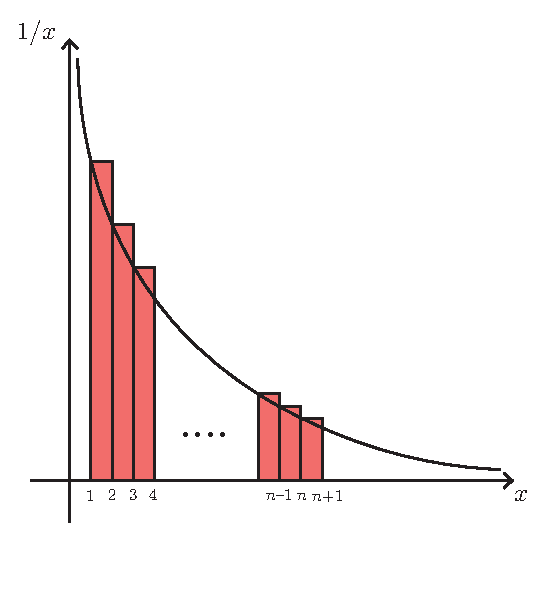
\includegraphics{figure1.eps}
\end{figure}\\
 上図のような求積を考えると、
\begin{align}
  \sum^{n}_{k=1}{\frac{1}{k}}>\int^{n+1}_{1}{\frac{1}{x}}\mathrm{d}x=\log{(n+1)}=\mathcal{O}(\log{n})
\end{align}
となる。
\begin{figure}[h]
  \centering
  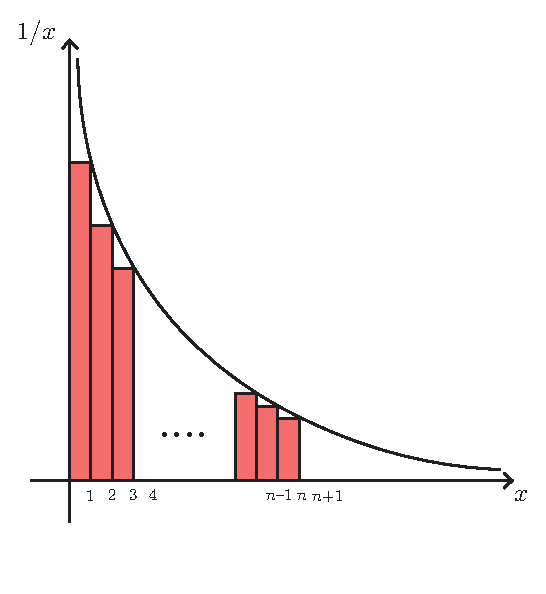
\includegraphics{figure2.eps}
\end{figure}\\
次に上図のような求積を考えると、
\begin{align}
  \sum^{n}_{k=1}{\frac{1}{k}}<1+\int^{n}_{1}{\frac{1}{x}}\mathrm{d}x=1+\log{(n)}=\mathcal{O}(\log{n})
\end{align}
となる。よって、(18)式と(19)式から、
\begin{align}
  \sum^{n}_{k=1}{\frac{1}{k}}=\mathcal{O}(\log{n})
\end{align}
となる。\\
\\
{\large\bfseries [発展問題03-01]}\\
 $a,b$を$a>b>1$となる整数とし、割り算
\begin{align*}
  a&=bq_1+r_1,\ 0<r_1<b\\
  b&=r_1q_2+r_2,\ 0<r_2<r_1\\
  &\hspace{5pt}\vdots\\
  r_{l-2}&=r_{l-1}q_l+r_l,\ r_{l-1}>r_l=0
\end{align*}
により整数$l$と$q_1,\cdots,q_l,r_1,\cdots,r_l$を定める。また、数列$\{F_n\}$をフィボナッチ数列とし、$\alpha$を$x^2=x+1$の解とする。\\
 まず、①$b\geq F_{l+1}$を示す。
\begin{align*}
  b&\geq r_1+r_2\\
  &\hspace{5pt}\vdots\\
  r_{k-2}&\geq r_{k-1}+r_k\ (2<k<l)\\
  &\hspace{5pt}\vdots\\
  r_{l-2}&>r_{l-1}>r_l=0
\end{align*}
が成り立つから、$r_{l-1}=1,r_{l-2}=2,\cdots,r_{k-2}=r_{k-1}+r_k,\cdots,b=r_1+r_2$のとき、つまり$b=F_{l+1}$のとき$b$は最小となる。よって、$b\geq F_{l+1}$である。\\
 次に②$F_{n+1}\geq{\alpha}^{n-1}$を数学的帰納法によって示す。\\
(i)\ $n=1,2$のとき、
\begin{align*}
  F_2=1,F_3=2>\frac{1+\sqrt{5}}{2}=\alpha
\end{align*}
が成り立つ。\\
(ii)\ $n=k,k+1\ (k:正の整数)$のとき$F_{n+1}\geq{\alpha}^{n-1}$が成り立つとする。このとき、${\alpha}^2=\alpha+1$であるから、
\begin{align*}
  F_{k+3}&=F_{k+1}+F_{k+2}\\
  &\geq{\alpha}^{k-1}+{\alpha}^k\\
  &={\alpha}^{k-1}\left(1+\alpha\right)\\
  &={\alpha}^{k-1}{\alpha}^2\\
  &={\alpha}^{k+1}
\end{align*}
となり、$n=k+2$のとき、$F_{n+1}\geq{\alpha}^{n-1}$が成り立つ。\\
(i)、(ii)から、すべての正の整数$n$に対して$F_{n+1}\geq{\alpha}^{n-1}$が成り立つ。\\
 最後に③${\alpha}^5>10$であることを示す。$\alpha=(1+\sqrt{5})/2$であるから、$(1+\sqrt{5})^5>10\cdot 2^5=320$を示せばよい。また、$(1+\sqrt{5})^5=176+80\sqrt{5}$より、$80\sqrt{5}>144$を示すことと等価となる。よって、$\left(80\sqrt{5}\right)^2=32000>20736=144^2$より、${\alpha}^5>10$が成り立つ。\\
 これらの公理から題意は示される。2つの整数$x,y$の最大公約数を$(x,y)$で表すと、
\begin{align*}
  (a,b)=(b,r_1)=\cdots=(r_{l-2},r_{l-1})=(r_{l-1}q_l,r_{l-1})=r_{l-1}
\end{align*}
であるから、$l\geq5d$を示せばよい。$b<10^d$と①、②を合わせると、
\begin{align*}
  {\alpha}^{l-1}\leq F_{l+1}\leq b<10^d
\end{align*}
が得られる。これと③を合わせると、
\begin{align*}
  10^{l-1}<{\alpha}^{5(l-1)}<10^{5d}
\end{align*}
となるから、$l-1<5d$つまり$l<5d+1$であり、$l\leq5d$が成り立つ。\\
\\
{\large\bfseries [発展問題03-02]}\\
 $a=r_0,b=r_1$と置く。このとき、$\mathrm{GCD}(a,b)=r=r_n$は次の式で与えられる。
\begin{align}
  r_0&=q_1r_1+r_2,\ 0<r_2<r_1\\
  r_1&=q_2r_2+r_3,\ 0<r_3<r_2\\
  r_2&=q_3r_3+r_4,\ 0<r_4<r_3\\
  &\hspace{5pt}\vdots\nonumber\\
  r_{k-1}&=q_kr_k+r_{k+1},\ 0<r_{k+1}<r_k\\
  &\hspace{5pt}\vdots\nonumber\\
  r_{n-2}&=q_{n-1}r_{n-1}+r_n,\ 0<r_n<r_{n-1}\\
  r_{n-1}&=q_nr_n
\end{align}
 このとき$i=0,1,2,\cdots,k$に対して、
\begin{align}
  ax_i+by_i=r_i
\end{align}
と表されたとすると、
\begin{align}
  x_{k+1}=x_{k-1}-q_kx_k\\
  y_{k+1}=y_{k-1}-q_ky_k
\end{align}
対して、
\begin{align}
  ax_{k+1}+by_{k+1}=r_{k+1}
\end{align}
が成立する。\\
 このことを証明する。まず、(24)式から
\begin{align}
  r_{k+1}=r_{k-1}-q_kr_k\nonumber
\end{align}
となるが、この右辺に(27)式の$i=k-1$と$i=k$のときを代入すると、
\begin{align}
  r_{k+1}&=\left(ax_{k-1}+by_{k-1}\right)-q_k\left(ax_k+by_k\right)\nonumber\\
  &=a\left(x_{k-1}-q_kx_k\right)+b\left(y_{k-1}-q_ky_k\right)\nonumber
\end{align}
この式に(28)、(29)式を代入すると、
\begin{align}
  r_{k+1}=x_{k+1}a+y_{k+1}b\nonumber
\end{align}
が得られる。\\
 ここで、$x_0=1,y_0=0,x_1=0,y_1=1$と置く。このとき、$a=r_0,b=r_1$と(21)、(22)式に注意すると、$i=0,1$に対して、
\begin{align*}
  ax_i+by_i=r_i
\end{align*}
が成立する。したがって、(27)、(28)、(29)、(30)式の操作を$k=2,3,\cdots,n-1$まで続けると、
\begin{align*}
  ax_n+by_n=r_n
\end{align*}
が得られる。ここで、$r_n=\mathrm{GCD}(a,b)=c$であるから、$x=x_n,y=y_n$と置くと、
\begin{align*}
  ax+by=c
\end{align*}
が得られる。\\
 $a=9876,b=5432$とき、ユークリッドの互除法から、
\begin{align*}
  9876&=5432\times1+4444\\[5pt]
  5432&=4444\times1+988\\[5pt]
  4444&=988\times4+492\\[5pt]
  988&=492\times2+4\\[5pt]
  492&=4\times123
\end{align*}
となり、GCD$(a,b)=4$とわかる。またこれより、数列$\{q_n\}\{x_n\}\{y_n\}$を求めると、
\begin{align*}
  \{q_n\}=\{1,1,4,2,123\}\\[5pt]
  \{x_n\}=\{1,0,1,-1,5,-11\}\\[5pt]
  \{y_n\}=\{0,1,-1,2,-9,20\}
\end{align*}
とわかる。これにより、求める$x,y$は、
\begin{align*}
  (x,y)=(-11,20)
\end{align*}
である。\\
\\
{\large\bfseries [発展問題04-01]}\\
 Pythonによってコードを作成すると次のようになる。
\begin{lstlisting}
  cache={}
  def tarai(x,y,z):
    if x<=y:
      return y
    key=(x,y,z)
    val=cache.get(key)
    if val != None:
      return val
    val=tarai(tarai(x-1,y,z),tarai(y-1,z,x),tarai(z-1,x,y))
    cache[key]=val
    return val
\end{lstlisting}
用いた工夫として、一度計算したTarai$(x,y,z)$については記憶しておき、2度と計算しないようにする点である。これを実装するためにPythonで辞書を用いた。\\
 これにより、
\begin{align*}
  \mathrm{Tarai}(20,10,0)=20
\end{align*}
となる。\\
\\
{\large\bfseries [発展問題06-01]}\\
\begin{align*}
  T(n)\leq\frac{1}{n}\sum^{n}_{i=1}\left\{T(i-1)+T(n-i)+c_1(n-1)\right\},\ (c_1>0)
\end{align*}
は、$\sum$の中身を計算することで、
\begin{align}
  T(n)\leq\frac{2}{n}\sum^{n-1}_{i=0}T(i)+c_1(n-1)
\end{align}
ここで、
\begin{align}
  T(n)\leq2n\ln{n}-\frac{c_1}{2}(n-1)
\end{align}
が成り立つことを帰納法を用いて示す。\\
(i)\ $n=1$のとき、$T(1)=0$で等号が成り立つことは自明である。\\
(ii)\ $k$以下の全ての正の整数$n\ (kは正の整数)$について、(32)式が成り立つと仮定すると、$n=k+1$のとき、
\begin{align}
  T(k+1)&\leq\frac{2}{k+1}\sum^{k}_{i=0}T(i)+c_1k\nonumber\\[5pt]
  &\leq\frac{2}{k+1}\sum^{k}_{i=1}\left\{2i\ln{i}-\frac{c_1}{2}(i-1)\right\}+c_1k+\frac{2}{k+1}T(0)\nonumber\\[5pt]
  &\leq\frac{4}{k+1}\int^{k+1}_{1}\left\{x\ln{x}-\frac{c_1}{2}(x-1)\right\}\mathrm{d}x+c_1k,\ (T(0)=0)\nonumber\\[5pt]
  &=\frac{4}{k+1}\left[\frac{x^2}{2}\ln{x}-\frac{x^2}{4}-c_1(x-1)^2\right]^{k+1}_1+c_1k\nonumber\\[5pt]
  &=2(k+1)\ln(k+1)-(k+1)-4c_1\frac{k^2}{k+1}+\frac{4}{k+1}+c_1k\nonumber\\[5pt]
  &=2(k+1)\ln(k+1)-\frac{(k+1)^2-4}{k+1}-2\frac{c_1}{2}k\left(\frac{4k}{k+1}-1\right)\nonumber\\[5pt]
  &<2(k+1)\ln(k+1)-\frac{c_1}{2}k
\end{align}
よって、$n=k+1$のときも成り立ち、(32)式は任意の正の整数$n$について成り立つ。すなわち、
\begin{align*}
  T(n)\leq2n\ln{n}-\frac{c_1}{2}(n-1)=\mathcal{O}(n\ln{n})
\end{align*}
より、$T(n)=\mathcal{O}(n\ln{n})$となる。





\end{document}
